\documentclass[11pt]{article}

\usepackage[margin=1in,letterpaper]{geometry}

\usepackage{graphicx}
\usepackage{float}
\usepackage{wrapfig}
\usepackage{amsmath}
\usepackage{parskip}

\linespread{1.2}

\renewcommand{\maketitle}{
    \begin{flushright}
        {\LARGE \textbf{CS763 Final Report: Contour interpolation by straight skeletons}}


    {\large \textsc{Wenhan Zhu (Cosmos)} \\ \textit{University of Waterloo}}
    \\ \today

    \end{flushright}
}

\begin{document}

\maketitle

\begin{abstract}
    Surface reconstruction for contours is very useful in the field of medical image analysis since only slices of information is available. The paper this report focuses on presents the first algorithm that gives an appealing result and guaranteed to have a valid surface.
\end{abstract}

\section{Introduction}
Surface reconstruction has become a popular problem since the digital era. Data acquired by equipments contain digitized data and reconstructing them is a interesting problem.

The paper this report is based on by Barequet {\it et al.} \cite{barequet04} provides the first algorithm that both guarantee a valid surface and provides a reasonable results. Previous attempt either assumes the input to be too simple or does not guarantee a correct surface output. It specifically focused on reconstructing surfaces of slices that is represented in contours.

The main idea of the paper is the same as previous work done by Oliva {\it et al.} \cite{oliva96} which defined an active region then use the straight skeleton (also called Angular Bisector Network at the time of Oliva's work) to separate the active region in to polygons. Then triangulate the polygons to create the surfaces. There are some differences between the work, the details is discussed in later sections.

\section{Difficulties of the problem}
Classified by Meyers {\it at el.} \cite{meyers91}, one of the main problem of 3D reconstruction is dealing with branching. (Figure \ref{fig:branching} from \cite{oliva96})

\begin{figure}[!h]
    \centering
        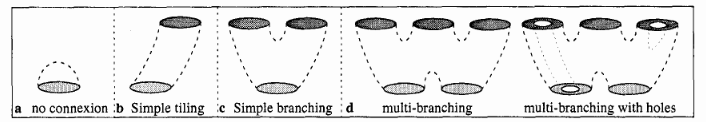
\includegraphics[width=0.8\textwidth]{branching.png}
        \caption{Different connections between layers}
        \label{fig:branching}
\end{figure}

Many of the previous work gave an triangulation between 2 consecutive surfaces, however, these triangulations does not guarantee a valid surface in general.

\section{Algorithm}

The algorithm the paper proposed is in 3 steps:

\begin{enumerate}
    \item Data processing
    \item Analyzing overlay of contours
    \item Compute the straight skeleton 
    \item Triangulate each region
    \item Lifting the vertices to create 3D surface
\end{enumerate}

\subsection{Data processing}
The only assumption for the input is that each contour is closed and for each layer, the contours are disjoint. My understanding for this is that in the application of the algorithm, medical images contain a lot of noise and computer vision algorithms at the time may not be able to produce good results on the contours. In a real life situations, a cut of a 3D polyhedral should always have the property which the algorithm assumes.

When we have each contours in a layer, we need to orient all the contours in a consistent way such that on the right of the contour is the "material". The paper mentions that in many situations, these information are given. If not the process of orienting the contours can be done by ordering them from outside layer to inner layer, the odd layers are clockwise, and the even layers are counter-clockwise which defines the "material" and "not-material" correctly. This process takes $O(n\log n)$ time.

\subsection{Analyzing overlay of contours}

By overlaying 2 layers of contours on the same plane, we can define the region where only exists in of the layers an active region. These regions are closed and the boundaries of these region can be described by the original sides of the polygon and 2 intersect points of each region created by intersections of the contours between 2 layers.

\subsection{Compute the straight skeleton}

Then we can compute the straight skeleton for each of the active regions. When computing the straight skeleton, we take notice of vertices created by 2 sides which belongs to contour sides of two layers and vertices created by sides which belong to the same layer. (Figure \ref{fig:straight-skeleton} from \cite{barequet04})

\begin{figure}[!h]
    \centering
        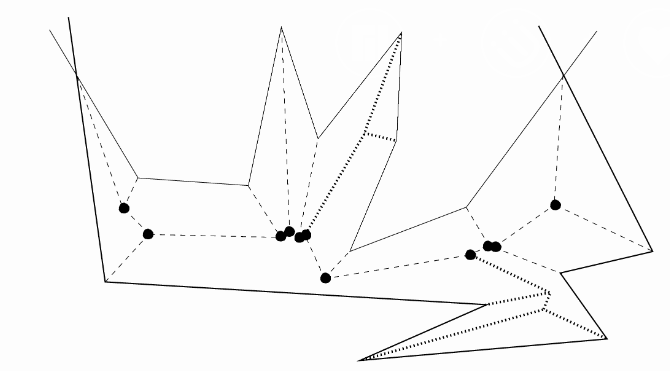
\includegraphics[width=0.8\textwidth]{straight-skeleton}
        \caption{Straight skeleton, highlighted vertices created by sides belong to 2 contours of different layer}
        \label{fig:straight-skeleton}
\end{figure}

One of the differences between Oliva's work and the paper's author work is here such that Oliva's algorithm can continue to subdivide each straight skeleton's region to subregions and create another straight skeleton. Oliva also mentioned that they considered generalised Voronoi diagrams of the region however, due to having parabola parts it's complicated to crease a version that only contain straight line segments.

\subsection{Triangulating each region}
The paper's authors uses the algorithm to triangulate a monotone polygon in $O(n)$ time. \cite[p.55~58]{cgaa} Each region of the straight skeleton is a monotone polygon with respect to each edge.

The other difference between Oliva's work and the authors is here. Oliva used another triangulation method that could create an overhanging structure which creates undesired final results.

\subsection{Lifting the vertices to create 3D surface}

With the straight skeleton and the triangulation done, we can lift the upper layer to 1, the lower layer remains 0. Then we lift the points on the straight skeleton and is created by contours of both layers to 0.5. Then the other vertices to the offset-distance from the edges. The offset distance is normalized to it's connecting distance to the straight skeleton. Offset-distance is described as the distance the polygon needs to shrink to reach the point.

The correctness of the surface is guaranteed by the triangulation method. We have the orientation of the contours, so we can procedurally calculate the orientation of each triangle and make sure they are facing the right direction.

This step takes $O(n^2)$ at worst time.

\section{Results}

The total time of the algorithm is bounded by the time needs to compute the straight skeleton. The worst case there could be $O(n^2)$ complexity to describe the active regions and a reasonable algorithm that computes the straight skeleton takes $O(k^2)$ where $k$ is the number of points. So the overall worst complexity of this algorithm is $O(n^4)$ with the specific implementation of computing straight skeleton.

\section{Later works}
With the evolution of digital world and improvements of technology, a discrete and simple interpolation is not enough. The authors of the paper later worked on a paper that sets to create a non-linear interpolation.\cite{barequet08} However, this paper is hidden behind a paywall so I did not have a change to look at it. Other work has been done on this with arbitrary slices by Bermano {\it et al.} \cite{bermano11}

Meanwhile, the development of 3D surface reconstruction of 3D point clouds and 3D point sets has been actively researched. Work by Kazhdan {\it at el.} \cite{kazhdan06} \cite{kazhdan13} showed promising results of reconstructing surfaces using {\it Poisson} approaches. Other methods are also popular. The main area of research seems to be done on the area of computer graphics.

\section{Conclusion}

Surface reconstruction has been a very active field. The advancement of technology has lead to many developments for different proposes. Traditional applications has moved from medical image analysis to more broad topics such as digitizing 3D objects. It is very interesting to see how the area will evolve in the following years with autonomous driving and other exciting technological advancements.


\bibliographystyle{unsrt}

\bibliography{sample}

\end{document}
